% ★★★ 难题
\newcommand{\qConicHardNationalBStem}{
已知椭圆 $E$ 的中心为坐标原点，对称轴为 $x$ 轴、$y$ 轴，且过 $A(0, -2)$，$B(\frac{3}{2}, -1)$ 两点．
(1) 求 $E$ 的方程；
(2) 设过点 $P(1, -2)$ 的直线交 $E$ 于 $M, N$ 两点，过 $M$ 且平行于 $x$ 轴的直线与线段 $AB$ 交于点 $T$，点 $H$ 满足 $\vec{MT} = \vec{TH}$．证明：直线 $HN$ 过定点．
}
\newcommand{\qConicHardNationalBFigure}{
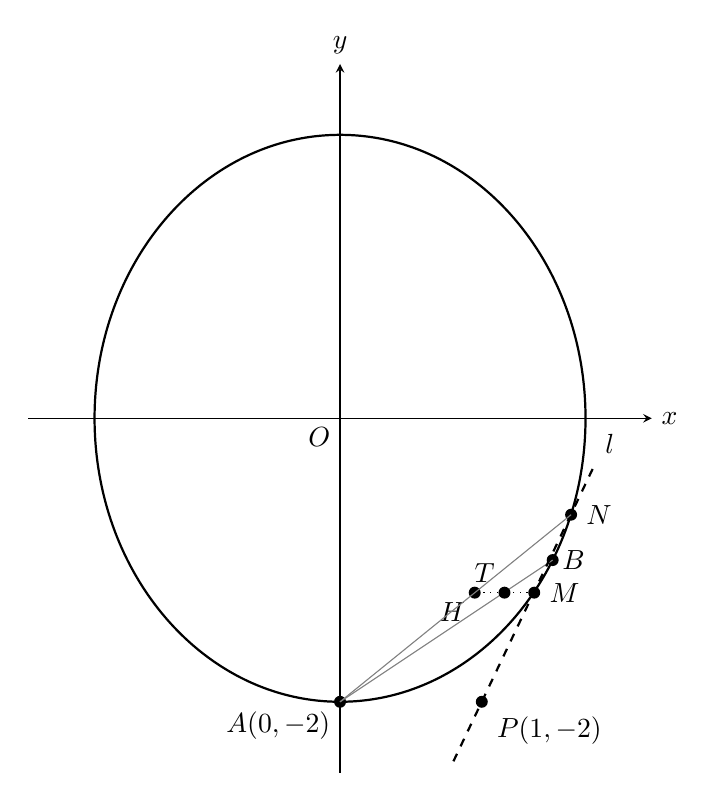
\begin{tikzpicture}[scale=1.8, >=stealth]
  % Axes
  \draw[->] (-2.2,0) -- (2.2,0) node[right] {$x$};
  \draw[->] (0,-2.5) -- (0,2.5) node[above] {$y$};
  \node[below left] at (0,0) {$O$};
  
  % Ellipse: x^2/3 + y^2/4 = 1 => vertical ellipse with a=2, b=1.732
  \draw[thick] (0,0) ellipse (1.732 and 2.0);
  
  % Points A(0, -2) and B(1.5, -1)
  \coordinate (A) at (0, -2.0);
  \coordinate (B) at (1.5, -1.0);
  \fill (A) circle (1.2pt) node[below left] {$A(0, -2)$};
  \fill (B) circle (1.2pt) node[right] {$B$};
  
  % Line segment AB
  \draw[thin, gray] (A) -- (B);
  
  % Point P(1, -2)
  \coordinate (P) at (1.0, -2.0);
  \fill (P) circle (1.2pt) node[below right, xshift=2pt, yshift=-2pt] {$P(1, -2)$};
  
  % Line l through P: y = 2.1(x - 1) - 2. Intersects ellipse at M and N.
  % M = (1.37, -1.23), N = (1.63, -0.68)
  \coordinate (M) at (1.37, -1.23);
  \coordinate (N) at (1.63, -0.68);
  \fill (M) circle (1.2pt) node[right, xshift=2pt] {$M$};
  \fill (N) circle (1.2pt) node[right, xshift=2pt] {$N$};
  
  \draw[thick, dashed] (0.8, -2.42) -- (1.8, -0.32) node[above right] {$l$};
  
  % Horizontal line through M(x1, y1)
  % T lies on AB: x_T = 1.5(y_M+2) = 1.16 => T(1.16, -1.23)
  \coordinate (T) at (1.16, -1.23);
  \fill (T) circle (1.2pt) node[above left] {$T$};
  \draw[dotted] (M) -- (T);
  
  % H satisfies T is midpoint of MH => x_H = 2x_T - x_M = 0.95 => H(0.95, -1.23)
  \coordinate (H) at (0.95, -1.23);
  \fill (H) circle (1.2pt) node[below left] {$H$};
  \draw[dotted] (T) -- (H);
  
  % Line HN passes through A(0, -2) and H(0.95, -1.23) and N(1.63, -0.68)
  \draw[thin, gray] (A) -- (N);
\end{tikzpicture}
}
\newcommand{\qConicHardNationalBAnswer}{
(1) 椭圆 $E$ 的方程为 $\frac{x^2}{3} + \frac{y^2}{4} = 1$．\\
(2) 证明见解析，直线 $HN$ 恒过定点 $A(0, -2)$．
}
\newcommand{\qConicHardNationalBSolution}{
\begin{proof*}
(1) 设椭圆 $E$ 的方程为 $mx^2 + ny^2 = 1$ ($m > 0, n > 0$)．\\
将点 $A(0, -2)$ 代入得：$4n = 1 \implies n = \frac{1}{4}$．\\
将点 $B(\frac{3}{2}, -1)$ 代入得：$\frac{9}{4}m + n = 1 \implies \frac{9}{4}m + \frac{1}{4} = 1 \implies m = \frac{1}{3}$．\\
所以椭圆 $E$ 的方程为 $\frac{x^2}{3} + \frac{y^2}{4} = 1$．\\

(2) 易知直线 $AB$ 的方程为 $y - (-2) = \frac{-1 - (-2)}{\frac{3}{2} - 0}(x - 0) \implies y + 2 = \frac{2}{3}x \implies x = \frac{3}{2}(y+2)$．\\
由题意，直线 $l$ 过点 $P(1, -2)$．且斜率显然不为 $0$，可设其方程为 $x = t(y+2) + 1$ ($t \in \mathbb{R}$)，一般式为 $x - ty - (2t+1) = 0$．\\
此时对应硬解系数为 $A=1, B=-t, C=-(2t+1)$．\\
在公式速查卡中，椭圆的标准方程为 $\frac{x^2}{a^2} + \frac{y^2}{b^2} = 1$．由于本题中椭圆为 $E: \frac{x^2}{3} + \frac{y^2}{4} = 1$，对应公式卡中的参数为 $a^2 = 3$（$x^2$ 的分母），$b^2 = 4$（$y^2$ 的分母）．\\
此时统一分母为 $D = A^2a^2 + B^2b^2 = 1^2(3) + (-t)^2(4) = 4t^2 + 3$．\\
联立直线与椭圆，消去 $x$ 整理得一元二次方程：
\[
(4t^2+3)y^2 + 8t(2t+1)y + 8(2t^2+2t-1) = 0
\]
根据相交充要条件 $D > C^2 \implies 4t^2+3 > (2t+1)^2 \implies 2t^2+2t-1 < \frac{3}{8}$，判别式 $\Delta > 0$ 成立．\\
设 $M(x_1, y_1), N(x_2, y_2)$，由硬解定理直接写出纵坐标的韦达公式，省去了常规代数联立并展开立式椭圆的冗长工作：
\[
y_1 + y_2 = -\frac{2BCb^2}{D} = -\frac{8t(2t+1)}{4t^2+3},\qquad y_1y_2 = \frac{b^2(C^2-A^2a^2)}{D} = \frac{8(2t^2+2t-1)}{4t^2+3}
\]
因为过 $M(x_1, y_1)$ 且平行于 $x$ 轴的直线为 $y = y_1$，与线段 $AB$ 交于点 $T(x_T, y_T)$，\\
所以 $y_T = y_1$．由于 $T$ 在直线 $AB$ 上，则其横坐标为 $x_T = \frac{3}{2}(y_1+2)$．\\
又因为 $\vec{MT} = \vec{TH}$，说明 $T$ 是线段 $MH$ 的中点，\\
所以点 $H(x_H, y_H)$ 的坐标满足：
\[
x_H = 2x_T - x_1 = 3(y_1+2) - x_1,\qquad y_H = y_T = y_1
\]
由于 $M(x_1, y_1)$ 在直线 $l$ 上，满足 $x_1 = t(y_1+2) + 1$，代入上式可得：
\[
x_H = 3(y_1+2) - [t(y_1+2)+1] = (3-t)(y_1+2) - 1
\]
下面证明直线 $HN$ 恒过定点 $A(0, -2)$．即证明 $H, N, A$ 三点共线，只需证明：
\[
\frac{y_2 - (-2)}{x_2 - 0} = \frac{y_1 - (-2)}{x_H - 0} \implies (y_2+2)x_H = (y_1+2)x_2
\]
我们将 $x_H = (3-t)(y_1+2) - 1$ 和 $x_2 = t(y_2+2) + 1$ 代入上式两端进行化简：
\[
\text{左端} = (y_2+2)[(3-t)(y_1+2) - 1] = (3-t)(y_1+2)(y_2+2) - (y_2+2)
\]
\[
\text{右端} = (y_1+2)[t(y_2+2) + 1] = t(y_1+2)(y_2+2) + (y_1+2)
\]
两端作差：
\[
\text{左端} - \text{右端} = (3-2t)(y_1+2)(y_2+2) - (y_1+y_2) - 4
\]
\[
= (3-2t)[y_1y_2 + 2(y_1+y_2) + 4] - (y_1+y_2) - 4
\]
由韦达定理，先算中括号部分：
\[
y_1y_2 + 2(y_1+y_2) + 4 = \frac{8(2t^2+2t-1) - 16t(2t+1) + 4(4t^2+3)}{4t^2+3}
\]
\[
= \frac{16t^2+16t-8 - 32t^2-16t + 16t^2+12}{4t^2+3} = \frac{4}{4t^2+3}
\]
代回差值表达式中：
\[
\text{左端} - \text{右端} = (3-2t)\left(\frac{4}{4t^2+3}\right) - \left(-\frac{8t(2t+1)}{4t^2+3}\right) - 4
\]
\[
= \frac{12-8t + 16t^2+8t - (16t^2+12)}{4t^2+3} = 0
\]
所以 $(y_2+2)x_H = (y_1+2)x_2$ 恒成立，即 $H, N, A$ 三点共线．\\
故直线 $HN$ 恒过定点 $A(0, -2)$．
\end{proof*}
}
\newcommand{\qConicHardNationalBDiagnosis}{
\errortag{定点猜测失误} 本题的难点之一在于“直线过定点”的定点需要由学生自行寻找。若采用特殊位置（如 $t=0$ 直线垂直 $x$ 轴）代入，可求得此时直线为 $y+2 = -\frac{y_1}{3y_1+4}x$，代入 $x=0$ 即可得 $y=-2$，锁定定点为 $A(0,-2)$．许多学生在没有特殊化定点时直接联立，极易在中途因为变量过多而放弃．\\
\errortag{代数化简繁琐} 在作差证明 $(3-2t)(y_1+2)(y_2+2) - (y_1+y_2) - 4 = 0$ 时，必须掌握“先整体计算其中一部分”的模块化化简意识（如本解析中先算 $y_1y_2+2(y_1+y_2)+4$）。若直接把韦达公式代入并通分，会导致代数项数过多，在限时紧张的情况下容易发生计算错误。
}
